\documentclass{article}
\usepackage{ctex}
\usepackage[utf8]{inputenc}
%\usepackage{natbib}
\usepackage[square,sort,comma,numbers]{natbib}
\usepackage{graphicx}
\usepackage{geometry}
 \usepackage{booktabs}
 \usepackage{siunitx}
\usepackage{listings}
\usepackage{subfigure}

\lstset{
    language=MATLAB,
    basicstyle=\ttfamily\small,
    aboveskip={1.0\baselineskip},
    belowskip={1.0\baselineskip},
    columns=fixed,
    extendedchars=true,
    breaklines=true,
    tabsize=4,
    prebreak=\raisebox{0ex}[0ex][0ex]{\ensuremath{\hookleftarrow}},
    frame=lines,
    showtabs=false,
    showspaces=false,
    showstringspaces=false,
    keywordstyle=\color[rgb]{0.627,0.126,0.941},
    commentstyle=\color[rgb]{0.133,0.545,0.133},
    stringstyle=\color[rgb]{01,0,0},
    numbers=left,
    numberstyle=\small,
    stepnumber=1,
    numbersep=10pt,
    captionpos=t,
    escapeinside={\%*}{*}
}

\usepackage{listings} % code display
\geometry{a4paper,centering,scale=0.8}
\usepackage[format=hang,font=small,textfont=it]{caption}
\usepackage[nottoc]{tocbibind}
\usepackage{float}
\usepackage{amsmath}

\usepackage[colorlinks=true, 
    linkcolor=blue,          % color of internal links
    citecolor=blue,        % color of links to bibliography
    filecolor=blue,      % color of file links
    urlcolor=blue]{hyperref}
    \usepackage[myheadings]{fullpage}

\numberwithin{equation}{subsection}
\newcommand{\HRule}[1]{\rule{\linewidth}{#1}}

\newcommand\degree{^\circ}
\date{}
%\bibliographystyle{plain}


\title{\heiti 复合光谱分峰模型}
\begin{document}
\maketitle
\begin{abstract}


针对问题一,首先建立以锚为原点、风向为$x$轴、竖直方向为$z$轴、海床所在平面为$O-xy$平面、风向所在铅垂面为$O-xz$平面的标准坐标系,从而刻画浮标的游动区域;其次,为描述系泊系统的状态,通过对该系统的各组成部分进行隔离受力分析,确定了浮标所受的杆拉力与风速、吃水深度的表达式。以及钢杆、钢桶、锚链倾角的递推关系,并结合海水深度的几何约束,最终建立了系泊系统状态模型;接着,基于锚链着地现象的考虑,对着地处的锚链进行了受力分析,从而得到了系泊系统状态的修正模型;最后,本文针对复杂多元非线性方程组的求解问题,设计了基于最小二乘法的搜索算法,求解出了海面风速分别为\SI{12}{m/s}和\SI{24}{m/s}时,钢桶和各节钢管的倾斜角度、锚链形状、浮标吃水深度与游动区域,见图XXX。

针对问题二,首先利用问题一建立的系泊系统状态模型和基于最小二乘法的搜索算法,对海面风速为\SI{36}{m/s}时,钢桶与各节
\\
\begin{flushleft}
\textbf{关键词:系泊系统}
\end{flushleft}
\end{abstract}


\newpage


\section{问题重述}


PCR (聚合酶链式反应)是一种用于放大扩增特定DNA片段的分子生物学技术,近年来广泛应用于核酸检测,可以大大提高检测的准确性和应用性。荧光定量PCR技术在PCR基础上引入了荧光基团,可以实时检测产物中的荧光信号,从而通过标准曲线对未知模板进行定量分析。实际在荧光信号的检测过程中,不同荧光基团产生的荧光具有不同的光谱范围,需要对荧光光谱进行区分。然而传统的区分方法使用了窄带滤光片,其透过光谱范围约为15-20nm较窄,会降低荧光信号的强度,从而降低检测的灵敏度。

所以,实现复合光谱分峰的方法,从采集的复合光谱曲线中分离不同荧光基团对应的光谱曲线,能够在保证灵敏度的同时对光谱进行区分,对于核酸检测技术及荧光定量PCR反应技术都具有重要意义。

\begin{itemize}
    \item 问题1:利用附件1中的数据建立双峰复合光谱的分峰模型,给出分峰后各峰的中心波长、高度及半峰宽,并计算得到的独立光谱曲线和原始曲线的线性相关系数。
    \item 问题2:分析在问题1的双峰分峰模型中,峰高比对所建立的分峰模型的影响。除使用赛题提供数据外,可使用虚拟数据仿真协助分析。
    \item 问题3:利用附件2中三峰和四峰叠加的光谱曲线及数据,建立多个光谱峰叠加的复合光谱曲线模型,将多峰复合光谱曲线拆分为独立光谱曲线(最多四个峰),并给出分离后各峰的中心波长、高度及半峰宽,与其相应的准单色光谱进行比较。
    \item 问题4:实际检测中的荧光光谱曲线多数是非对称的光谱曲线。利用附件3中实际的检测数据尝试建立非对称光谱曲线分峰的数学模型,将复合光谱曲线拟合拆分为对应的独立光谱曲线。
\end{itemize}



\section{问题假设}
1.假设复合光谱的形成仅与各独立光谱有关。由于复合光谱的荧光信号强度较大,检测灵敏度较高,外界环境对数据造成的干扰可以忽略不计。

2.假设实验数据允许存在一定的误差范围。由于测量精度的限制,数据会有一定误差。

3.假设叠加光谱均满足瑞利判据。题目中给出的多波峰叠加的复合光谱应当是可以分峰的。



\section{问题分析}
\subsection{问题一的分析}
问题一要实现双峰复合光谱的分峰模型,并给出各峰的中心波长,高度及半峰宽。首先对单峰光谱曲线进行曲线拟合,由光谱形成原理可以推得:单峰光谱的峰强与波长满足高斯函数分布。然后根据
\subsection{问题二的分析}

为了计算海面风速为为\SI{36}{m/s}时,钢桶和各节钢管的倾斜角度、锚链形状和浮标的游动区域,则只要将海面风速代入模型一进行求解即可。

为了满足钢桶的倾斜角度不超过\SI{5}{°},锚链在锚点与海床的夹角不超过\SI{16}{°}的要求,需要建立以重物配重为决策变量,海水深度为几何约束条件的多目标非线性规划模型。由于数据规模不大,本文采用循环搜索算法对模型进行求解。

\subsection{问题三的分析}
为了分析在海水深度、海水速度、风速变化情况下钢桶、钢管的倾斜角度、锚链形状、浮标吃水深度与游动区域,需要根据问题二的思路建立多目标非线性规划模型,决策变量为锚链型号、锚链长度及重物配置。

\subsection{问题四的分析}







\section{符号说明}
\begin{table}[H]
    \centering
    \begin{tabular}{c|c}
\hline
符号&解释\\
\hline
$\delta$&控制器单元之间的距离$(mm)$\\
$D$&圆的直径$(mm)$\\
$\Delta N$&附件中上边界与下边界的行坐标之差(格)\\
$m$&总计投影数据组数\\
$I$&射线强度\\
$I_0$&入射X光强度\\
$l$&穿透物体厚度\\
$\mu$&衰减系数\\
$\beta$&处理前的吸收率\\
$\beta^{'}$&处理后的吸收率\\
$\alpha$&增益系数\\			
$\Delta n_i$&附件中第i组数据的上边界与下边界的行坐标之差(格)\\
$\theta$&旋转角\\
$A$&垂足值\\
$S$&投影点数值之和\\
$a$&椭圆长半轴长度\\
$b$&椭圆短半轴长度\\
$\varepsilon$&误差值\\
\hline
    \end{tabular}
    \caption{符号说明}
    \label{tab:my_label}
\end{table}


\section{问题一模型的建立与求解}
\subsection{模型准备}
对于本问题,可通过引入决策变量浮标吃水深度$h$,以海面风速和海水深度$H$在作为已知条件,借助物理学与力学原理进行机理分析得到系统内在关系,进而求得系泊系统各状态参数。

首先,本文以锚和锚链的交点为原点,建立空间直角坐标系来讨论系统内部的受力情况,示意图如图\ref{坐标系}:
\begin{figure}[H]
  \centering
  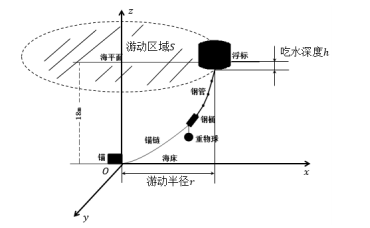
\includegraphics[scale=0.6]{1.png}
  \caption{\zihao{-5}\kaishu 系统空间坐标系}
  \label{坐标系}
\end{figure}

接着,为了方便表述,我们用$P_{1}$\textasciitilde $P_{N}$依次表示系统内部从上到下的$N$种构建,由题中锚链长度除以单个链环的长度可以得到锚链共有210个链环,由此得到$N$的数值:
$$N=1+4+1+210+1=218$$

各编号代表的具体构建如\ref{构件编号}下表所示:
\begin{table}[!htbp]
\centering
    \begin{tabular}{|c|c|c|c|c|c|}
\hline
编号$P_{i}$ & $i=1$&$2\le i\le5$&$i=6$&$7\le i\le216$&$i=217$\\
\hline
构件类型&浮标&钢管&钢桶&锚链&锚\\
\hline
    \end{tabular}
    \caption{各构件编号}
    \label{构件编号}
\end{table}




\subsection{模型建立}
\subsubsection{系泊系统受力分析}
本文假设风向平行于海平面,当风速度不变时,海风方向的变化会使浮标在圆形区域内运动,并且各方向平衡时系统状态相同。因此,本文在平面内对系统进行受力分析。

\begin{flushleft}
\textbf{(一)浮标的受力}
\end{flushleft}
如图\ref{浮标受力}所示,浮标受到速度为$v$的海风作用在海面上达到平衡,设其吃水深度为$h$,此时浮标一共受到4个力的作用。

\begin{figure}[H]
  \centering
  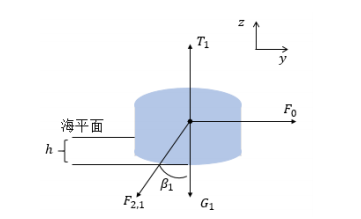
\includegraphics[scale=0.6]{2.png}
  \caption{浮标受力示意图}
  \label{浮标受力}
\end{figure}
其中$T_{1}$表示浮标所受浮力大小,方向竖直向上。由阿基米德定律可得到浮力$T_{1}$与吃水深度$h$的关系为
\begin{equation}
    T_{1}=\rho g\cdot\frac{\pi d_{1}^{2}h}{4}
\end{equation}
式中,$\rho$为海水的密度;$d_{1}$为浮标底面直径。

浮标还受到水平方向的风力$F_{0}$的作用,由题中已知关系式可知风力和风速有如下关系:
\begin{equation}
\begin{cases}
F_{0}=0.625\times S_{1}v^{2}\\
S_{1}=(l_{1}-h)d_{1}
\end{cases}
\end{equation}
其中$S_{1}$为浮标在风向法平面的投影面积,$l_{1}$为浮标高度。

浮标下表面与第一节钢管铰接,钢管对浮标作用力的大小用$F_{2,1}$表示,其与竖直方向的夹角为$\beta_{1}$。此外,物体还受到竖直向下的重力$G_{1}$。物体受力平衡根据牛顿第一定律有浮标在$x,y$方向的合力为零,即:
\begin{equation}
\begin{cases}
F_{0}-F_{2,1}\sin\beta_{1}=0\\
T_{1}-F_{2,1}\cos\beta_{1}=G_{1}
\end{cases}
\end{equation}



\begin{flushleft}
\textbf{(二)钢管的受力}
\end{flushleft}
\begin{figure}[H]
  \centering
  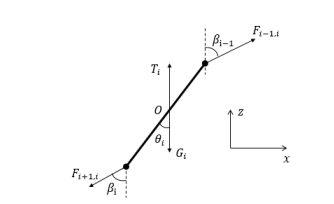
\includegraphics[scale=0.6]{钢管受力.png}
  \caption{\zihao{-5}\kaishu 钢管受力示意图}
  \label{钢管受力}
\end{figure}

钢管$P_{i}(2\le i\le5)$受力如图\ref{钢管受力}所示

\begin{flushleft}
\textbf{(三)钢桶的受力}
\end{flushleft}

如图\ref{钢桶受力}所示,钢桶静止时共受到6个外力作用,其倾斜角度(与竖直方向夹角)为$\theta_{6}$,其上端与钢管$P_{5}$铰接,钢管对钢桶作用力大小为$F_{5,6}$,倾角为$\beta_{5}$;下端与锚链链环$P_{8}$铰接并悬挂一重物球,链环对钢管作用力大小为$F_{8,6}$,倾角为$\beta_{6}$。
\begin{figure}[H]
  \centering
  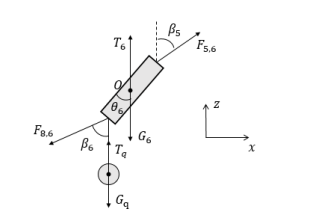
\includegraphics[scale=0.6]{钢桶受力.png}
  \caption{\zihao{-5}\kaishu 钢桶受力示意图}
  \label{钢桶受力}
\end{figure}

首先,同样由阿基米德定律得到钢桶浮力$T_{6}$与重物球浮力$T_{q}$表达式如下:
\begin{equation}
\begin{cases}
T_{6}=\rho g\cdot\frac{\pi d_{6}^{2}l_{6}}{4}\\
T_{q}=\rho g\cdot m_{q}\rho_{q}
\end{cases}
\label{式子}
\end{equation}
式中,$d_{6},i_{6}$分别为钢桶的底面直径和轴向高度;$m_{q},\rho_{q}$分别为重物球的质量和密度。

\begin{flushleft}
\textbf{(四)锚链的受力}
\end{flushleft}

锚链各节链环的受力情况与各节钢管受力情况相似,因此上文中的钢管递推关系同样适用于锚链链环。但对于链环浮力的计算,题中只给出了各节链环的质量,体积是未知的,本文参考题目背景中“采用无档普通链环”查阅资料。


\subsubsection{系泊系统几何约束分析}
根据以上受力分析,系泊系统状态由决策变量浮标吃水深度$h$确定,可通过海床深度约束对其进行求解。
\begin{figure}[H]
  \centering
  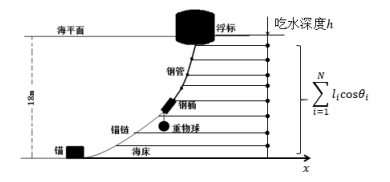
\includegraphics[scale=0.6]{构建投影.png}
  \caption{\zihao{-5}\kaishu 构建投影示意图}
  \label{构建投影}
\end{figure}

如图\ref{构建投影}所示,系统稳定时在海水中各构件在竖直方向上的投影总长度应该等于海床深度,即
\begin{equation}
    h+\sum_{i=1}^{N}l_{i}\cos\theta_{i}=H
\end{equation}

由各构件在水平方向上的投影长度进一步得到浮标游动圆半径$r$:
\begin{equation}
r=\sum_{i=1}^{N}l_{i}\sin\theta_{i}
\end{equation}

综合以上分析得到系泊系统的状态模型总的表述为:

\begin{equation}
F_{2,1}=\dfrac{\sqrt{25(l_{1}-h)^{2}d_{1}v^{4}+4(\rho g\pi dh-4G_{1})}}{8}
\end{equation}

\begin{equation}
\beta_{1}=\arctan\dfrac{5(l_{1}-h)d_{1}v^{2}}{8G_{1}+2g\rho\pi d_{1}^{2}h}
\end{equation}

\begin{equation}
\beta_{6}=\arctan\frac{F_{5,6}\sin\beta_{5}}{F_{5,6}\cos\beta_{5}+T_{6}+T_{q}-G_{6}-G_{q}}
\end{equation}

\begin{equation}
F_{8,6}=\frac{F_{5,6}\sin\beta_{5}}{\sin(\arctan\dfrac{F_{5,6}\sin\beta_{5}}{F_{5,6}\cos\beta_{5}+T_{6}+T_{q}-G_{6}-G_{q}})}
\end{equation}

\begin{equation}\left\{\begin{array}{l}
F_{2,1}=\dfrac{\sqrt{25\left(l_{1}-h\right)^{2} d_{1} v^{4}+4\left(\rho g \pi d h-4 G_{1}\right)}}{8} \\
\quad \\
\beta_{1}=\arctan \dfrac{5\left(l_{1}-h\right) d_{1} v^{2}}{8 G_{1}+2 g \rho \pi d_{1}^{2} h}
\end{array}\right.\end{equation}

\begin{equation}\left\{\begin{array}{l}
G_{p i p e}+F_{4} \cos \gamma_{4}=f_{p i p e}+F_{5} \cos \gamma_{5} \\
F_{4} \sin \gamma_{4}=F_{5} \sin \gamma_{5} \\
F_{4} L \sin \left(\gamma_{4}-\theta_{4}\right)=F_{5} L \sin \left(\theta_{4}-\gamma_{5}\right)
\end{array}\right.\end{equation}

\begin{equation}\begin{array}{l}
y=\frac{F_{\text {wind }}}{\sigma g} \cosh \left\frac{\sigma g}{F_{\text {wind }}} x+\sinh ^{-1}\left(\tan \alpha_{1}\right)\right-\frac{F_{\text {wind }}}{\sigma g} \cosh \left(\sinh ^{-1}\left(\tan \alpha_{1}\right)\right) \\
\Rightarrow y=\frac{F^{\prime}}{\sigma g} \cosh \left(\frac{\sigma g}{F^{\prime}} x+\sinh ^{-1}\left(\tan \alpha_{1}\right)\right)-\frac{F^{\prime}}{\sigma g} \cosh \left(\sinh ^{-1}\left(\tan \alpha_{1}\right)\right)
\end{array}\end{equation}

\subsection{模型修正}
在实际情况中,当风速过小时锚链会提前沉底,导致以上模型对于锚链链环作用力与倾角的递推关系不再适用,因此本文针对这一情况对模型进行修正。示意图如图所示
\begin{figure}[H]
  \centering
  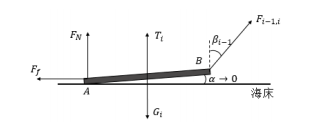
\includegraphics[scale=0.6]{完全沉底.png}
  \caption{\zihao{-5}\kaishu 完全沉底链环受力示意图}
  \label{完全沉底}
\end{figure}

由图\ref{完全沉底}可知,锚链第一个完全沉底的链环共受到5个外力的作用,分别为重力$G_{i}$,浮力$T_{i}$,摩擦力$F_{f}$,海床提供的支撑力$F_{N}$以及上一个链环的拉力$F_{i-1,i}$。

在链环处于将要被提起处于临界状态时,其与海床的夹角$\alpha\to0^{+}$,对$A$点取矩有:

综上所述,对模型作出如下修正:
\begin{itemize}
    \item 增加海水中构建竖直方向受力约束:$\displaystyle \sum_{j=1}^{i-1}T_{j}-G_{j}\le0.5(G_{i}-T_{i})$。
    \item 更改锚链递推关系式适用范围:$7\le i\le j$,$j$表示第一个脱离海床链环的编号。
    \item 更改浮标游动半径表达式:$\displaystyle r=\sum_{i=1}^{j}l_{i}\sin\theta_{i}+\sum_{i=j+1}^{216}l_{i}$。
\end{itemize}
至此,针对链环沉底情况对模型修正完毕。

\subsection{模型求解}
对于系泊系统状态模型的求解,难以直接通过大量状态方程得到定解,所以联立非线性方程组求定解方法不适用。因此本文采用一种基于最小二乘思想的循环搜索算法对模型进行求解。

\subsubsection{基于最小二乘思想的循环搜索算法}
描述系泊系统状态模型中的未知变量包括吃水深度$h$,钢桶,各节钢管以及锚链刚体的倾斜角度$\theta_{i}$,由模型可确定各个倾斜角度度$\theta_{i}$与钢桶吃水深度$h$的递推关系,故倾斜角度可由钢桶的倾斜角度确定,故风速$v$确定的情况下,系泊系统的状态可由吃水深度$h$一个变量确定。因此将吃水深度$h$为连续变量,故将其离散化进行定步长搜索可对模型进行求解,具体算法步骤如图\ref{流程图}所示:
\begin{figure}[H]
  \centering
  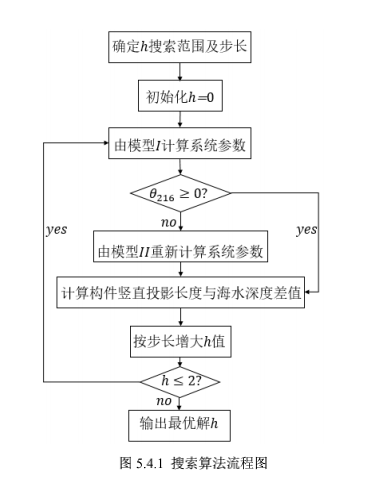
\includegraphics[scale=0.6]{流程图.png}
  \caption{\zihao{-5}\kaishu 搜索算法流程图}
  \label{流程图}
\end{figure}

图\ref{流程图}中,模型为未修正模型,模型为针对锚链提前触底修正后的模型。

\subsubsection{算法精度检验}
对于定步长的循环搜索算法,误差的主要来源为变量的步长,因此可以通过减小步长,根据最优解变化幅度来判断步长是否合理。

取变量$h$步长为原步长的$\frac{1}{50}$,则算法精度因提高50倍,定义相对优化量$q$为目标函数优化量与理论优化量的比值:
$$q=\frac{|S'(h)-S(h)|}{50}$$

通过MATLAB编程计算可得$q=0.38\times10^{-3}$,由于长度范围在0.1数量级,因此$q$可以忽略不计,故目前搜索算法中设置的步长可认为是合理的。

\subsubsection{结果分析}
本文假设锚链和重物球材料为普通铸铁,其密度为$7.8\times10^{3}kg/m^{3}$,由此参数求解。

当海面风速为\SI{12}{m/s}时,本文通过MATLAB编程对模型进行求解。结果表明此时锚链出现提前触底的情况,此时各构件倾角与浮标吃水深度如表\ref{求解结果1}所示:
\begin{table}[!htbp]
\centering
    \begin{tabular}{c|c}
\hline
钢桶倾角&1.2089°\\
\hline
钢管1倾角&1.1641°\\
\hline
钢管2倾角&1.1720°\\
\hline
    \end{tabular}
    \caption{求解结果}
    \label{求解结果1}
\end{table}

由于锚链提前沉底,本文假设沉底锚链完全拉直,得到浮标游动半径为14.7232m,进而得到游动区域面积为\SI{681}{m^{2}},在$xoy$平面表达式为$x^{2}+y^{2}\le681$,单位为m。此时锚链从第152个链环开始触底,沉底链环个数为59个,锚链形状及各构件在$x0z$坐标平面中形状如图\ref{锚链1}所示:
\begin{figure}[H]
    \begin{minipage}[c]{0.5\textwidth}
        \centering
        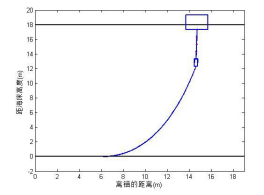
\includegraphics[width=0.7\textwidth]{锚链1.png}
        \caption{\zihao{-5}\kaishu 锚链形状示意图}
        \label{锚链1}
    \end{minipage}
    \begin{minipage}[c]{0.5\textwidth}
        \centering
        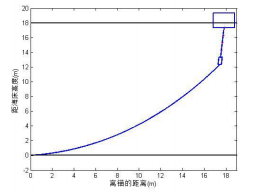
\includegraphics[width=0.7\textwidth]{锚链2.png}
        \caption{\zihao{-5}\kaishu 锚链形状示意图}
        \label{锚链2}
    \end{minipage}
\end{figure}

当海面风速为\SI{24}{m/s}时,求解结果表明此时锚链完全脱离海床没有提前触底。求解得到系统各参数如表\ref{求解结果2}所示:
\begin{table}[!htbp]
\centering
    \begin{tabular}{c|c}
\hline
钢桶倾角&4.5837°\\
\hline
钢管1倾角&4.4294°\\
\hline
钢管2倾角&4.458°\\
\hline
    \end{tabular}
    \caption{求解结果}
    \label{求解结果2}
\end{table}

浮标游动半径\SI{17.8224}{m},得到其游动区域面积为\SI{997.89}{m^{2}},在$xoy$平面表达式为$x^{2}+y^{2}\le997.89$,单位为m。此时锚链在锚点与海床夹角为5.7059°,求解得到锚链形状如图\ref{锚链2}所示。

\section{问题二模型的建立与求解}
\subsection{模型准备}
本问题首先要根据问题一中模型计算海面风速为\SI{36}{m/s}时系统的各个状态参数。接着题目要求通过调节重物球的质量来使钢桶倾角和锚链在锚点与海床的夹角小于给定阈值,由此可以通过问题一模型计算得到重物球的质量范围,但结合题目背景考虑,本文建立优化模型,在满足约束范围内搜索重物球的最优质量使得系统达到最优状态。

\subsection{系泊系统优化模型的建立}
\begin{flushleft}
\textbf{(一)决策变量的确定}
\end{flushleft}
根据题目要求,本文假设重物球材料不变,确定重物球的质量$m_{q}$为模型的决策变量,通过调节$m_{q}$的大小来对目标进行优化。

\begin{flushleft}
\textbf{(二)目标函数分析}
\end{flushleft}
由题目背景可知,要对系泊系统进行优化就要使得浮标的吃水深度和游动区域以及钢桶的倾斜角度尽可能小。据此本位一共确立如下三个优化目标:
\begin{itemize}
\item 钢桶的倾斜角度尽可能小:
$$\min\theta_{6}=\arctan\frac{F_{5,6}\sin\beta_{5}}{0.5(T_{6}-G_{6})+F_{5,6}\cos\beta_{5}}$$
\item 浮标的吃水深度尽可能小:
$$\min h=H-\sum_{i=1}^{N}l_{i}\cos\theta_{i}$$
\item 浮标的在海面上的游动区域为圆形,目标可以转化为浮标的游动半径尽可能小:
$$\min r=\sum_{i=1}^{N}l_{i}\sin\theta_{i}$$
\end{itemize}

\begin{flushleft}
\textbf{(三)约束条件分析}
\end{flushleft}

问题二同样满足问题一的假设,因此优化模型需要满足问题一模型的约束条件。此外根据题目要求,还需要满足锚链在锚点与海床夹角不超过16°:
\begin{equation}
    \frac{\pi}{2}-\theta_{216}\le16°
\end{equation}

式中$\theta_{216}$为锚点相连接的链环与竖直方向的夹角。此外,对于优化目标钢桶的倾角$\theta_{6}$还需满足约束:
\begin{equation}
    \theta_{6}=\arctan\frac{F_{5,6}\sin\beta_{5}}{0.5(T_{6}-G_{6})+F_{5,6}\cos\beta_{5}}\le
\end{equation}

综合以上分析,并结合问题一模型中系统中各构件作用力与倾角的递推关系得到系泊系统的优化模型为:

\subsection{模型求解}
\subsubsection{多目标转化单目标求解}
对于三个目标的权重值的确定,基于赋权的可靠性考虑,本文在此选择了主观性相对较小,能够充分利用数据特征的熵权法。熵权法可以根据各个目标的变异度,利用信息熵计算出各个目标的客观权重值。信息熵越小,变异程度最大,重要程度越大。期计算结果为$A=11.46,B=1.5,C=0.05$

接着我们对以上三个目标分别赋以权重$A,B,C$,将多目标转化为单目标的优化问题,用$U$表示总的优化目标:
$$\min U=A\cdot\theta_{6}+B\cdot h+C\cdot r$$

\subsubsection{风速为\SI{36}{m/s}时系统参数解}
通过MATLAB编程代入风速对问题一模型进行求解,结果表明此时锚链全部浮于水中,此时各构件倾角与浮标吃水深度如表\ref{求解结果3}所示:
\begin{table}[!htbp]
\centering
    \begin{tabular}{c|c}
\hline
钢桶倾角&9.4767°\\
\hline
钢管1倾角&9.1822°\\
\hline
钢管2倾角&9.2375°\\
\hline
    \end{tabular}
    \caption{求解结果}
    \label{求解结果3}
\end{table}

得到浮标游动半径为\SI{18.8906}{m},进而得到游动区域面积为\SI{1121.092}{m^{2}},其在$xoy$平面表达式为$x^{2}+y^{2}\le1121.092$。此时,锚链在锚点与海床的夹角大小为21.397°>16°,表明锚点被拖动。锚链在$x0z$坐标平面中形状如图\ref{锚链4}所示:
\begin{figure}[H]
  \centering
  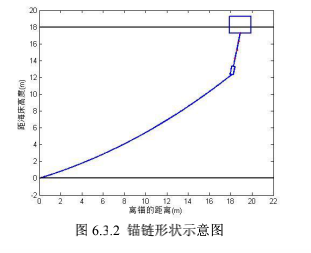
\includegraphics[scale=0.6]{锚链4.png}
  \caption{\zihao{-5}\kaishu 锚链形状示意图}
  \label{锚链4}
\end{figure}

\subsubsection{系泊系统优化模型的求解}
\begin{flushleft}
\textbf{(一)循环搜索算法求解}
\end{flushleft}

Step1:根据系泊系统的设计要求求解重物球的质量范围$m_{q_{\min}}$\textasciitilde $m_{q_{\max}}$,令重物的初始重量值为质量范围下限$m_{q_{\min}}$;

Step2:将重物球最小质量$m_{q}$代入模型一,按照模型一的求解算法求解出并记录此时的吃水深度$h$,钢桶倾斜角度$\theta_{6}$,锚链在锚点与海床夹角$90°-\theta_{216}$,浮标游动半径$r$,并求解出此时的目标函数值$u$,并令$\min u=u$。

Step3:判断此时的系统状态是否满足$90°-\theta_{216}\le16°,\theta_{6}\le5$的约束条件,若满足进入Step4,不满足进入Step5;

Step4:若$u\le\min u$,则令$\min u=u$,并记录$h,\theta_{6},r$,否则$\min u$保持不变。

Step5:令$m_{q}=m_{q}+0.5$;

Step6:若$m_{q}\le m_{q_{\max}}$,返回Step2,否则结束程序,输出$h,\theta_{6},r$。

\begin{flushleft}
\textbf{(二)结果分析}
\end{flushleft}

根据以上算法,通过MATLAB程序求解,得到满足题目要求时重物球的质量范围,并在此范围内求得重物球的最佳质量,是的系统达到最优状态,结果如表所示

\begin{flushleft}
\textbf{(三)灵敏度分析}
\end{flushleft}

为进一步研究重物球质量变化对每个优化目标的相关性及相关程度,我们对模型进行灵敏度分析,结果下图所示
\begin{lstlisting}

\end{lstlisting}



\newpage
\begin{thebibliography}{99}
	\bibitem{1}乐经良,向隆万,李世栋. 数学实验[M],股票期权定价的Black-Scholes方程和二叉树方法
	\bibitem{2}许艺铧.股票期权定价模型应用研究——以A公司为例[J].中外企业家,2018(24):188-189.
    \bibitem{3}程志勇. 混合高斯模型下美式期权定价及风险度量[D].兰州财经大学,2018.
    \bibitem[]{4}陈丽,林玲.具有时滞效应的股票期权定价[J].山东大学学报(理学版),2018,53(04):36-41.
    \bibitem[]{5}Jean-Guy Simonato. American option pricing under GARCH with non-normal innovations[J]. Springer US,2019,20(3).
    \bibitem[]{6}Rui Gao,Yaqiong Li,Lisha Lin. Bayesian statistical inference for European options with stock liquidity[J]. Elsevier B.V.,2019,518.
\end{thebibliography}

\end{document}
